\chapter{Time Series Clustering}

\subsubsection*{What is a time series}
In this report we will deal with \textit{discrete time series}. 
A time series is defined as a set of observations $\{x_t\}$ recorded at a specific time $t$. 
A discrete time series is a time series where the set of times when observations are made ($T_0$) is discrete \cite{brockwell_davis_advanced}. 
A multivariate time series can be viewed as a set of vectors $\{\mathbf{x}_t\}$ where each set of vector elements $\{x^i_t\}$ is an individual time series. 
This means that the elements of the same vector $[x^1_t, x^2_t,...,x^N_t]$ are separate observations made at the same time instance $t$. 
In a wind turbine, measurements of the temperature in the gear box made every 10 seconds can be considered a univariate time series. 
While the set of measurements made every 10 seconds of the temperature in the gear box, the power produced by the turbine, and the wind speed ahead of the blades can be considered a multivariate time series. \bigskip

\section{Overview of Time Series Clustering}
There are three types of TSC, \textit{whole-series TSC}, \textit{subsequence TSC} and \textit{time-point TSC}. 
Whole-series TSC is when multiple ''whole'' time series are clustered with respect to each other. 
Subsequence TSC comprises the clustering of subsequences of the same time series with respect to each other. 
The defining difference between whole-series and subsequence TSC is that whole-series TSC clusters multiple time series while subsequence TSC clusters clusters different subsequences of the same time series. 
When performing time-point TSC the goal is to cluster individual observations of a time series wrt. to each other. 
In this review we will only consider work using whole-series TSC, so when the phrase \textit{time-series clustering} is used, one can assume that whole-series TSC is what is being refered to. \bigskip

TSC can be divided into three distinct parts: representation method, similarity metric and clustering algorithm. 
The choice of representation is key, and is the task of retaining the valuable information while disregarding the irrelevant information. As mentioned in section \ref{sec:intro}, only feature extraction based, and model based representation methods will be considered. 
The choice of similarity metric is important, as it decides which aspects of the time series will be used to measure (dis)similarity. 
Requirements for similarity metric is especially important in the raw-data, and feature based clustering approaches. 
In the model-based clustering approach they can be relaxed as the representation method already limits the number of aspects which one can compare time series with. 
Choice of distance metric also has a significant impact on the time-complexity of the clustering system. 

%% SMAL SECTION ABOUT RAW-DATA BASED APPROACH, FEATURE BASED APPROACH AND MODEL BASED APPROACH.

\section{Representation Methods}
There are numerous ways which a time series can be represented. 
\textcite{tsc_rev} define a time series representation given time series data $\{x_t\} = \{x_1, x_2, ... ,x_T\}$ as transforming the time series into another vector $\{x_t\} = \{\hat{x}_1, \hat{x}_2, ... ,\hat{x}_L\}$ where $L < T$. 
In theory $L=T$, but most often the point in transforming a time series is to reduce the amount of information present in the raw time series to more easily reveal patterns of interest. 
% \input{tsc/rep_methods.tex}
In the following subsections the theory of the three most prevalant feature extraction methods, and time series models will be presented: ARMA models, HMM and PCA.
Then the different representation methods encountered in the literature will be discussed.

\subsection{Time Series Models and Representations} \label{sec:ts_models}
To select suitable mathematical models for a dataset, we have to allow for the random nature of future observations. 
This is done by assuming that each observation in a time series $x_t$ is a realization of a particular random variable $X_t$. 
The time series can then be modelled as a collection/set of random variables $\{X_t\}$, also known as a \textit{stochastic process} \cite{brockwell_davis_advanced}. 

\subsubsection*{Autoregressive Moving Average Models}
To define an ARMA model, one needs to have a clear understanding of the terms white noise process, and stationary process. 
We say that the stochastic process $\{Z_t\}$ is ''white noise'' with zero mean, and variance $\sigma^2$ ($\{Z_t\} \sim WN(0, \sigma^2)$) if and only if $\{Z_t\}$ is zero mean, and every random variable contained in $\{Z_t\}$ is uncorrelated with every other random variable contained in $\{Z_t\}$. 
A stochastic process $\{X_t\}$ is said to be weakly wide-sense stationary if the mean, and variance are constant for all terms in the process. 
$\{X_t\}$ is said to be weakly short-term stationary if the mean and variance of terms are constant for distinct time periods within the duration of the process, but are not constant for all terms in the process. 
For brevity the term ''stationary process'' will be used when refering to a \textit{weakly wide-sense stationary process}. 
An ARMA model descirbes a time series in terms of difference equations. 
It can be considered a combination of two smaller models, an autoregressive (AR) model and a moving average (MA) model. 
Let $\{X_t\}$ be a stationary process. 
An $\mathrm{MA}(q)$ model will describe every term $X_t$ as a linear combination of $q$ distinct white noise terms as in equation \eqref{eq:MA_q}.

\begin{equation}
    X_t = Z_{t} + \theta_1 Z_{t-1} + ... + \theta_q Z_{t-q}
    \label{eq:MA_q}
\end{equation}

Whereas an $\mathrm{AR}(p)$ model will describe every term $X_t$ as a linear combination of $p$ previous terms of $\{X_t\}$ as in equation \eqref{eq:AR_p}

\begin{equation}
    X_t = \phi_1 X_{t-1} + ... + \phi_p X_{t-p}
    \label{eq:AR_p}
\end{equation}

Putting equations \eqref{eq:AR_p} and \eqref{eq:MA_q} together, an $\mathrm{ARMA}(p,q)$ model will describe every term $X_t$ as a linear combination of $p$ previous terms, and $q$ white noise terms as in equation \eqref{eq:ARMA_p_q}.

\begin{equation}
    X_t - \phi_1 X_{t-1} - ... - \phi_p X_{t-p} = Z_{t} + \theta_1 Z_{t-1} + ... + \theta_q Z_{t-q}
    \label{eq:ARMA_p_q}
\end{equation}

Given that the polynomials $1 + \theta_1 z + \theta_2 z^2 + ... + \theta_q z^q$ and $1 - \phi_1 z - \phi_2 z^2 - ... - \phi_p z^p$ have no common factors \cite{brockwell_davis}.

\subsubsection*{Hidden Markov Models} \label{s:hmm}
Let $\{X_n\}$ be a stochastic process where the random variables contained in $\{X_n\}$ only can take on a finite number of values which we will call states. 
Let $X_n$ denote the state at time period $n$. 
The probability of $X_n$ transitioning from state $i$ to state $j$ at the next time period $n+1$ is called the transition probability, and is denoted $p_{ij}$. 
It seems natural that $p_{ij}$ is conditional on what the state has been in previous time periods. 
$\{X_t\}$ is said to be a \textit{Markov chain} if $p_{ij}$ only is conditional on the past state, as shown in equation \eqref{eq:markov_property}.

\begin{equation}
    \begin{split}
        p_{ij}  &= P(X_n = i | X_{n-1} = i_{n-1}, X_{n-2} = i_{n-2},..., X_{1} = i_{1}, X_{0} = i_{0}) \\
                &= P(X_n = i | X_{n-1} = i_{n-1})      
    \end{split}
    \label{eq:markov_property}
\end{equation}

Suppose now that the states that the process is in are hidden from the observer. 
Instead there exists a finite set of signals $\{S\}$ that are emmitted when the process enters a state. 
For each state there is a set of \textit{emission probabilities} $P(S = s | X = j)$ associeted with a subset of the signals that can be emmitted.
In addition, let the probability of emmitting signal $s$, at time period $n$, in state $j$ ($P(S_n = s | X_n = j)$) be independent of previous states, and signals emmitted. 
A model of this type where the signals $S_1, S_2, ...$ are observed, and the underlying Markov states remain hidden is called a \textit{hidden Markov model} \cite{stoch_pros}. 

\subsubsection*{Principal Component Analysis and Independent Component Analysis}
There are two ways of reducing dimensionality in classification and regression tasks. 
One can choose to only use a subset of the dimensions given, or one can use a combination of the dimensions given.
PCA and ICA are both tools that reduce dimensionality by using a linear combination of the original dimensions given.
Consider a multivariate time series represented by the matrix $X$ with $n$ columns, where each column is a univariate time series of length $m$.
$X$ can then be reduced to a matrix of fewer columns of the same length by multiplying it with a projection matrix $W$, as in equation \ref{eq:reduce}. 
Let $Z$ represent the reduced matrix.
In PCA, the columns of $Z$ are called the \textit{principal components}, and in ICA they are called the \textit{independent components}. 

\begin{equation}
    Z = W X
    \label{eq:reduce}
\end{equation}

PCA and ICA is are methods for choosing $W$. 
In PCA $W$ is chosen in such a manner that the resulting dimensions are the dimensions with the highest variance.
The principal components are in fact the eigenvectors of the covarience matrix of $X$, so all the principal components are orthogonal. 
This is best illustrated graphically as in figure \ref{fig:pca_illustrated} where $w_1$ and $w_2$ illustrate the first and second principal components respectively.

\begin{figure}
    \begin{center}
    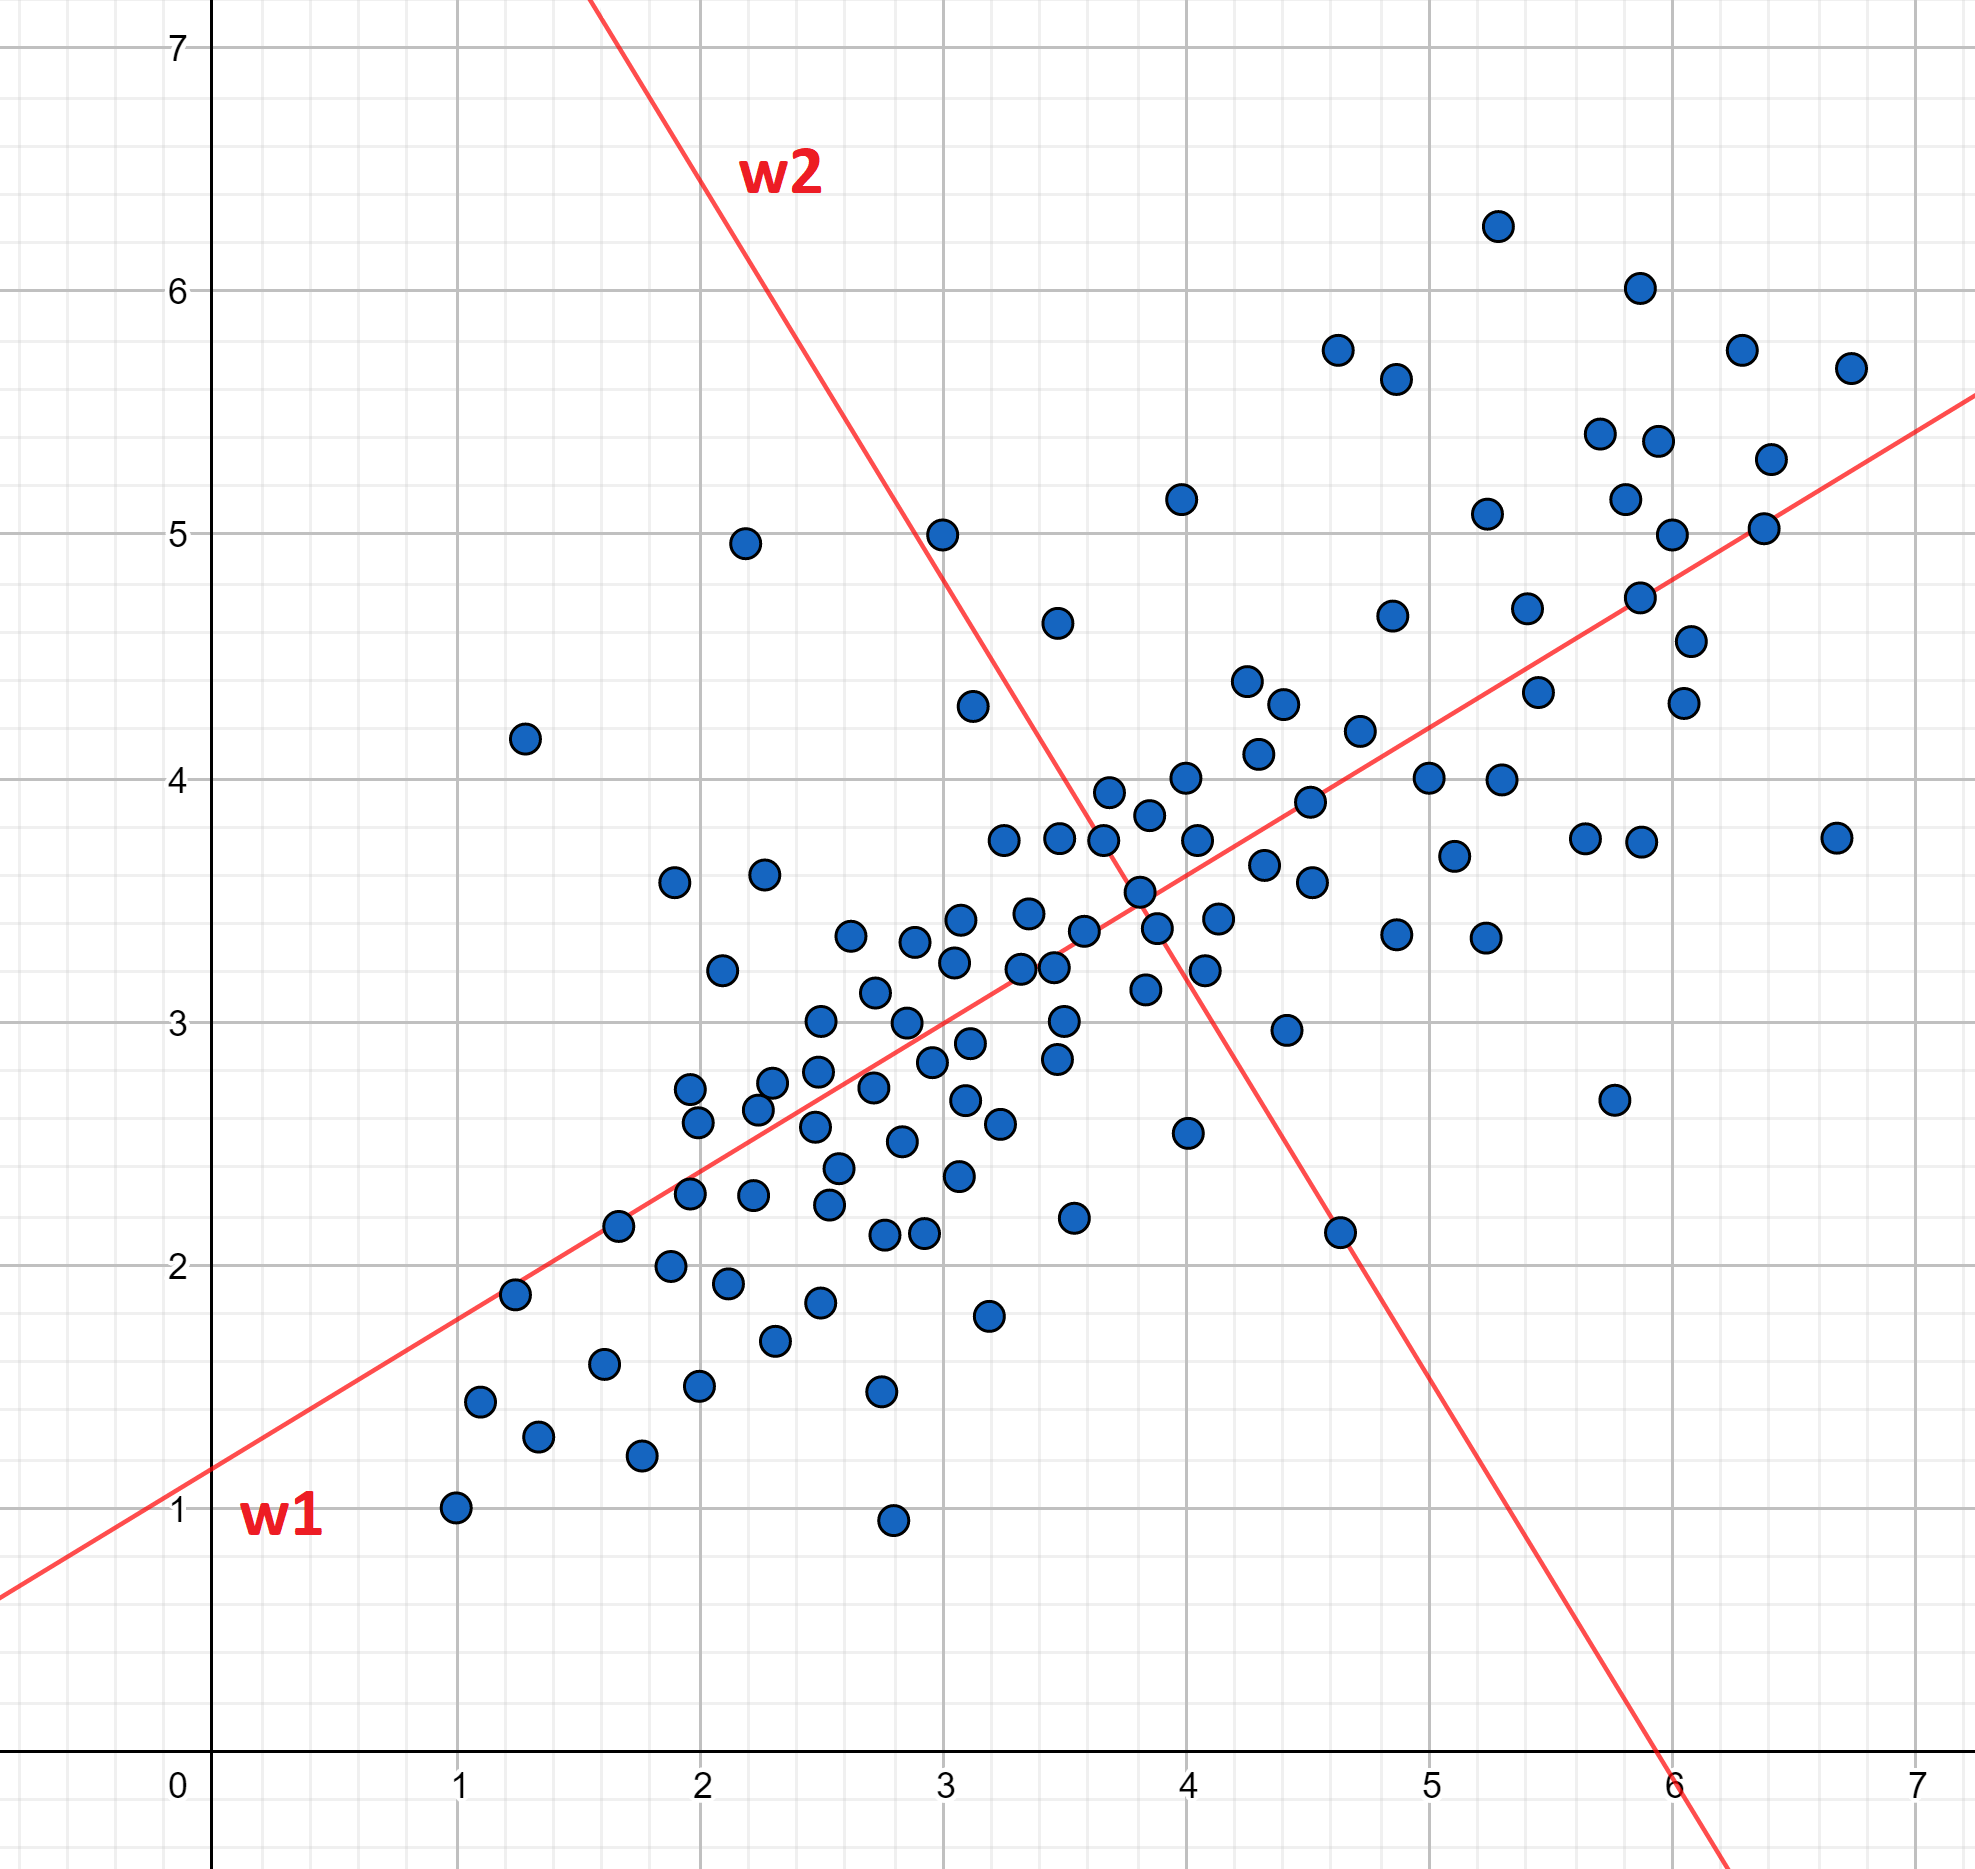
\includegraphics[width=0.4\textwidth]{tsc/pca_illustrated.png}
    \end{center}
    \caption{Illustration of how the principal components are found} 
    \label{fig:pca_illustrated}
\end{figure}

In ICA one assumes that the matrix of observed variables is a linear combination of mutually independent variables with an addition of noise, as illustrated in equation \ref{eq:ica_basics}. 
Where $X$ is the matrix of observed variables, $S$ is the matrix of independent hidden variables, $A$ is called a ''mixing matrix'' and $E$ is a noise matrix.  

\begin{equation}
    X = A S + E
\end{equation}

ICA is based upon the central limit theorem which states that a sum of random variables with arbitrary probability distributions will tend towards a Gaussian distribution. 
Hence, one chooses $W$ such that the resulting independent components are mutually independent and show as little Gaussian properties as possible.

\subsection{Feature Extraction Based Representations}

\begin{table*}[h]
    \centering
    \ra{1.3}
    \begin{tabular}{p{0.45\textwidth}p{0.3\textwidth}}
        \toprule
        Feature extraction method & Articles \\
        \midrule
        PCA or ICA.                             & \cite{hysteresis_tsc_tensor_decomp, road_grade_china_pca_kmeans, load_tsc_state_space_model, multivariate_tsc_common_pca, ica_tsc_sea_level, copula_ica_tsc} \\
        Time-frequency decomposition.           & \cite{shape_feat_mod_tsc_rfa, wavelet_multivar_tsc_multi_pca, ambient_air_vape_k_means, dwt_hac_kmeans_som, xml_dft_delaunay_traingulation, tsc_total_variation_distance, fragmented_periodogram, BSLEX_nonlin_nonstat_tsc}  \\
        % Wavelet transform.                    & \cite{shape_feat_mod_tsc_rfa, wavelet_multivar_tsc_multi_pca, ambient_air_vape_k_means, dwt_hac_kmeans_som, } \\
        % DFT.                                  & \cite{xml_dft_delaunay_traingulation, } \\
        % Spectral densities.                   & \cite{tsc_total_variation_distance} \\
        % Fragmented periodogram.               & \cite{fragmented_periodogram, } \\
        % BSLEX.                                & \cite{BSLEX_nonlin_nonstat_tsc} \\
        Signal statistics.                      & \cite{ghsom_optimal_hedge_ratio, tsc_slaughterhouse, road_grade_china_pca_kmeans, auto_encoder_many_tsc_algorithms, } \\
        Matrix, or tensor decomposition.        & \cite{multivar_tsc_riemann_manifold, fuzzy_c_means_pso_svd, svd_birch_tsc_stock_price, hysteresis_tsc_tensor_decomp, tensor_multi_elastic_kernel_tsc} \\
        % Covarience matrices.                  & \cite{multivar_tsc_riemann_manifold, } \\
        % Singular value decomposition (SVD).   & \cite{fuzzy_c_means_pso_svd, svd_birch_tsc_stock_price, } \\
        % Tensor decomposition.                 & \cite{hysteresis_tsc_tensor_decomp, tensor_multi_elastic_kernel_tsc} \\
        Symbolic aggregate approximation (SAX). & \cite{clust_large_datasets_aghabozorg, apxdist_sax_k_modes, shape_feat_mod_tsc_rfa} \\
        Permutation based coding.               & \cite{dependency_tsc_energy_markets} \\
        Spline functions.                       & \cite{hier_clust_w_state_space_models} \\
        Topological feature extraction.         & \cite{topology_for_shape_based_tsc, } \\
        Autoencoder.                            & \cite{auto_encoder_many_tsc_algorithms} \\
        \bottomrule
    \end{tabular}
    \caption{Feature extraction based representation methods.}
    \label{tab:feat_repr_meth}
\end{table*}

\subsection{Model Based Representations}

\begin{table*}[h]
    \centering
    \ra{1.3}
    \begin{tabular}{p{0.45\textwidth}p{0.3\textwidth}}
        \toprule
        Time series model & Articles \\
        \midrule
        HMM.                                    & \cite{mixture_gaussian_hmm, hmm_pm10_quantifying_impacts, multivariate_tsc_hmm} \\
        ARMA model.                             & \cite{garch_robust_tsc, shape_feat_mod_tsc_rfa, temporal_tsc_threshold_ar_models, tsc_ar_metric_air_pollution, ar_metric_trimmed_fuzzy_tsc_pm10, moar_mpl_tsc, struct_damage_ar_fuzzy_c_means, fstar_hac_tsc, var_multivar_tsc} \\  
        State space model.                      & \cite{stock_price_tsc_regr_trees_som, load_tsc_state_space_model} \\
        Varience ratio statistics.              & \cite{financial_tsc_variance_ratio, } \\
        Copula based model.                     & \cite{copula_fuzzy_tsc_spatial} \\
        Network model.                          & \cite{community_detection_networks_tsc, multivar_tsc_community_detection, } \\
        \bottomrule
    \end{tabular}
    \caption{Model based representation methods}
    \label{tab:model_repr_meth}
\end{table*}

\section{Similarity Metrics}
One similarity metric is Euclidean distance.
Another similarity metric is dynamic time warping.

\begin{table*}[h]
    \centering
    \ra{1.3}
    \begin{tabular}{p{0.45\textwidth}p{0.3\textwidth}}
        \toprule
        Similarity Metric & Articles \\
        \midrule
        Euclidean distance.                 & \cite{financial_tsc_variance_ratio, hier_clust_w_state_space_models, topology_for_shape_based_tsc, community_detection_networks_tsc, shape_feat_mod_tsc_rfa, multivar_tsc_riemann_manifold, temporal_tsc_threshold_ar_models, ar_metric_trimmed_fuzzy_tsc_pm10, copula_ica_tsc, tsc_slaughterhouse, ambient_air_vape_k_means, dwt_hac_kmeans_som, xml_dft_delaunay_traingulation, svd_birch_tsc_stock_price, road_grade_china_pca_kmeans, fragmented_periodogram, auto_encoder_many_tsc_algorithms, load_tsc_state_space_model, struct_damage_ar_fuzzy_c_means, var_multivar_tsc} \\
        Squared Euclidean distance.         & \cite{garch_robust_tsc, } \\
        Exponential Euclidean distance.     & \cite{tsc_ar_metric_air_pollution, load_tsc_state_space_model, } \\
        P-norms.                            & \cite{community_detection_networks_tsc, copula_fuzzy_tsc_spatial} \\
        Minkowski distance.                 & \cite{shape_feat_mod_tsc_rfa,} \\
        Tensor distance metric.             & \cite{hysteresis_tsc_tensor_decomp, } \\
        Matrix $L^p$ norms                  & \cite{tensor_multi_elastic_kernel_tsc} \\
        Dynamic time warping distance (DTW).& \cite{community_detection_networks_tsc, shape_feat_mod_tsc_rfa, temporal_tsc_threshold_ar_models} \\
        Approximate distance (APXDIST).     & \cite{clust_large_datasets_aghabozorg, apxdist_sax_k_modes} \\
        MINDIST.                            & \cite{shape_feat_mod_tsc_rfa, } \\
        Haussdorf distance.                 & \cite{temporal_tsc_threshold_ar_models, } \\
        Aggregated quasi-distance.          & \cite{BSLEX_nonlin_nonstat_tsc, } \\
        Kullback-Leibler distance.          & \cite{multivariate_tsc_hmm, } \\
        Total variation distance.           & \cite{tsc_total_variation_distance, } \\
        PCA similarity metric.              & \cite{wavelet_multivar_tsc_multi_pca} \\
        Information based metrics.          & \cite{dependency_tsc_energy_markets, } \\
        Pearson correlation coefficient.    & \cite{community_detection_networks_tsc, shape_feat_mod_tsc_rfa, fuzzy_c_means_pso_svd, } \\
        Test statistics.                    & \cite{fstar_hac_tsc, } \\
        Principal component $R_e$.          & \cite{multivariate_tsc_common_pca} \\
        \bottomrule
    \end{tabular}
    \caption{}
    \label{tab:}
\end{table*}

\section{Clustering Algorithms}
As mentioned before clustering is a form of unsupervised machine learning. 
The goal is to divide the dataset into clusters, by maximizing some similarity metric for members of the same cluster, and minimizing the same metric for members of different clusters.

\begin{table*}[h]
    \centering
    \ra{1.3}
    \begin{tabular}{p{0.45\textwidth}p{0.3\textwidth}}
        \toprule
        Clustering Algorithm & Articles \\
        \midrule
        Expectation maximization 			& \cite{mixture_gaussian_hmm, moar_mpl_tsc, auto_encoder_many_tsc_algorithms} \\
        Hierarchical clustering 			& \cite{financial_tsc_variance_ratio, hier_clust_w_state_space_models, BSLEX_nonlin_nonstat_tsc, shape_feat_mod_tsc_rfa, ica_tsc_sea_level, multivar_tsc_riemann_manifold, tsc_total_variation_distance, dependency_tsc_energy_markets, copula_ica_tsc, tsc_slaughterhouse, dwt_hac_kmeans_som, auto_encoder_many_tsc_algorithms, fstar_hac_tsc, } \\
        K-means family 						& \cite{financial_tsc_variance_ratio, hier_clust_w_state_space_models, topology_for_shape_based_tsc, multivariate_tsc_hmm, apxdist_sax_k_modes, temporal_tsc_threshold_ar_models, ambient_air_vape_k_means, hysteresis_tsc_tensor_decomp, dwt_hac_kmeans_som, road_grade_china_pca_kmeans, auto_encoder_many_tsc_algorithms} \\
        Fuzzy C-means family 				& \cite{garch_robust_tsc, copula_fuzzy_tsc_spatial, temporal_tsc_threshold_ar_models, tsc_ar_metric_air_pollution, wavelet_multivar_tsc_multi_pca, ar_metric_trimmed_fuzzy_tsc_pm10, fuzzy_c_means_pso_svd, struct_damage_ar_fuzzy_c_means, } \\
        Self-organizing map (SOM) 			& \cite{ghsom_optimal_hedge_ratio, stock_price_tsc_regr_trees_som, dwt_hac_kmeans_som, } \\
        State space model 					& \cite{hier_clust_w_state_space_models, } \\
        Community detection algorithms		& \cite{community_detection_networks_tsc, } \\
        Custom algorithms 					& \cite{clust_large_datasets_aghabozorg, multivariate_tsc_common_pca, tensor_multi_elastic_kernel_tsc, var_multivar_tsc} \\
        Spectral clustering 				& \cite{temporal_tsc_threshold_ar_models, fragmented_periodogram, auto_encoder_many_tsc_algorithms, } \\
        Matrix factorization 				& \cite{multivar_tsc_community_detection} \\
        Delauney Triangulation method 		& \cite{xml_dft_delaunay_traingulation} \\
        BIRCH 								& \cite{svd_birch_tsc_stock_price, auto_encoder_many_tsc_algorithms, } \\
        Affinity propagation  				& \cite{auto_encoder_many_tsc_algorithms} \\
        DBSCAN  							& \cite{auto_encoder_many_tsc_algorithms} \\
        Mean shift  						& \cite{auto_encoder_many_tsc_algorithms} \\
        \bottomrule
    \end{tabular}
    \caption{Clustering algorithms}
    \label{tab:clust_alg}
\end{table*}

\section{Discussion}
